\documentclass[tikz,border=7pt]{standalone}
\usepackage{amsmath,amssymb}
\usepackage[scaled]{helvet}
\renewcommand{\familydefault}{\sfdefault}
\usetikzlibrary{arrows.meta,backgrounds,calc,fit,positioning,shapes.geometric}
\definecolor{bpink}{HTML}{172033}
\definecolor{bpblue}{HTML}{2A78D6}
\definecolor{bporange}{HTML}{E56A32}
\definecolor{bpgreen}{HTML}{168A65}
\definecolor{bppurple}{HTML}{7A5CC7}
\definecolor{bpred}{HTML}{C94A4A}
\definecolor{bpmuted}{HTML}{667085}
\definecolor{bpgrid}{HTML}{D8DEE8}
\definecolor{bpsurface}{HTML}{F8FAFC}
\tikzset{
  var/.style={circle,draw=bpblue,fill=bpblue!10,line width=.9pt,minimum size=8mm,font=\small\bfseries,text=bpink},
  factor/.style={rectangle,rounded corners=1.5pt,draw=bporange,fill=bporange!14,line width=.9pt,minimum size=6.8mm,font=\small\bfseries,text=bpink},
  constraint/.style={rectangle,rounded corners=1.5pt,draw=bpred,fill=bpred!12,line width=.9pt,minimum size=6.8mm,font=\small\bfseries,text=bpink},
  edge/.style={draw=bpmuted!75,line width=.9pt},
  msgvf/.style={-{Latex[length=2.2mm]},draw=bpblue,line width=1.35pt},
  msgfv/.style={-{Latex[length=2.2mm]},draw=bporange,line width=1.35pt},
  label/.style={font=\scriptsize,text=bpmuted,align=center},
  title/.style={font=\bfseries\large,text=bpink},
  card/.style={draw=bpgrid,fill=bpsurface,rounded corners=7pt,line width=.7pt},
}

\begin{document}
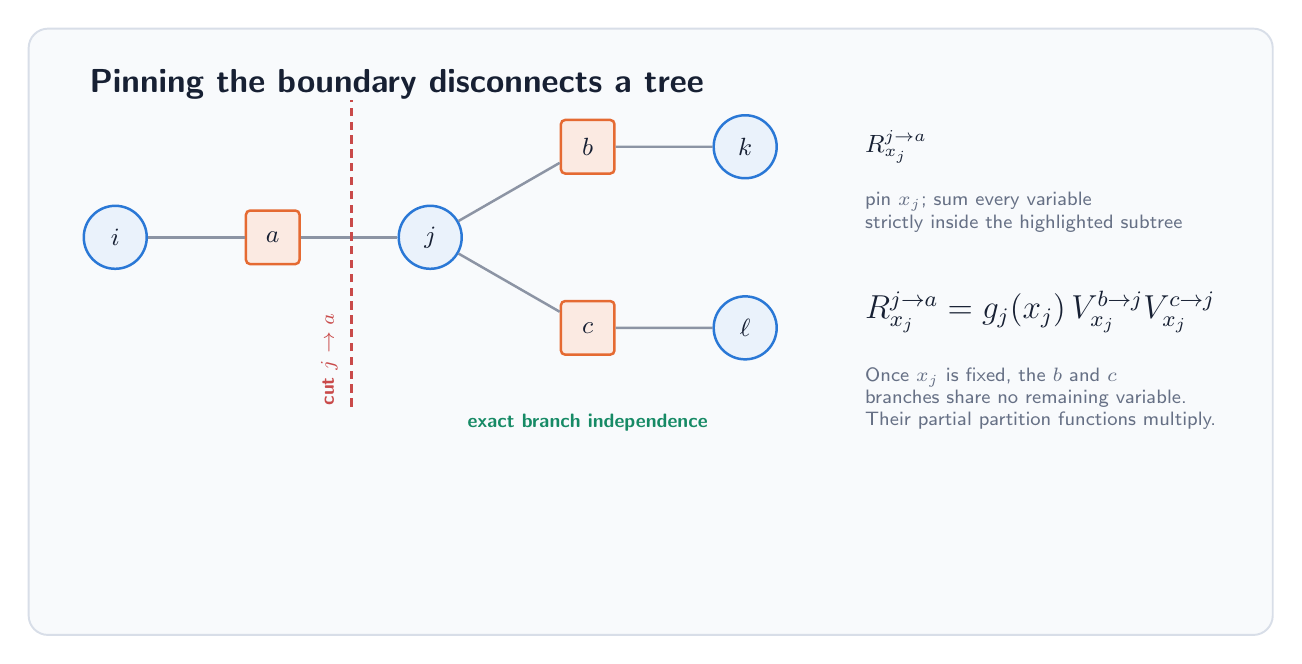
\begin{tikzpicture}[font=\sffamily]
  \node[card,minimum width=15.8cm,minimum height=7.7cm] at (6.8,2.2) {};
  \node[title,anchor=west] at (-.45,5.35) {Pinning the boundary disconnects a tree};
  \begin{scope}[on background layer]
    \filldraw[draw=bpred,fill=bpred!7,rounded corners=6pt,line width=.7pt]
      (3.25,1.55) rectangle (8.75,5.15);
  \end{scope}
  \node[var] (i) at (0,3.4) {$i$};
  \node[factor] (a) at (2,3.4) {$a$};
  \node[var] (j) at (4,3.4) {$j$};
  \node[factor] (b) at (6,4.55) {$b$};
  \node[factor] (c) at (6,2.25) {$c$};
  \node[var] (k) at (8,4.55) {$k$};
  \node[var] (l) at (8,2.25) {$\ell$};
  \draw[edge] (i)--(a)--(j);
  \draw[edge] (j)--(b)--(k);
  \draw[edge] (j)--(c)--(l);
  \draw[bpred,densely dashed,line width=1.2pt] (3,1.25)--(3,5.15);
  \node[text=bpred,font=\scriptsize\bfseries,rotate=90] at (2.72,1.85) {cut $j\to a$};
  \node[anchor=west,text=bpink,font=\small] at (9.4,4.55) {$R^{j\to a}_{x_j}$};
  \node[anchor=west,label,align=left] at (9.4,3.72) {pin $x_j$; sum every variable\\strictly inside the highlighted subtree};
  \node[anchor=west,text=bpink,font=\large] at (9.4,2.45) {$R^{j\to a}_{x_j}=g_j(x_j)\,V^{b\to j}_{x_j}V^{c\to j}_{x_j}$};
  \node[anchor=west,label,align=left] at (9.4,1.35) {Once $x_j$ is fixed, the $b$ and $c$\\branches share no remaining variable.\\Their partial partition functions multiply.};
  \node[text=bpgreen,font=\scriptsize\bfseries] at (6,1.05) {exact branch independence};
\end{tikzpicture}
\end{document}
